\renewcommand*\chapterpagestyle{scrheadings}
\chapter{Implementation and Issues}

\section{Spring Boot Prototype}
\subsection{Backend implementation}
The backend service was initially implemented in Kotlin using Spring Boot \footnote{The Spring Framework \cite{spring}},
a Java-based framework that provides core infrastructure support for web applications.
The service exposed a prototype REST endpoint at http://localhost:8080/process,
which accepted textual input as a preliminary alternative to audio processing.
The endpoint implemented pattern matching to route weather-related queries to a weather service,
while other queries were processed through the GPT-4 language model.

\subsection{HTTP client in Qt}
The initial prototype consisted of a minimal user interface
implementing three basic components arranged vertically:
a QLineEdit widget for text input,
a QPushButton for submission,
and a QLabel to display the server's response.
The button's \texttt{clicked()} signal was connected to a slot
handling the network communication.
When the submit button was clicked, the application sent a POST request
to \texttt{http://localhost:8080/process} containing the user's input as plain text,
and asynchronously processed the server's response through Qt's signal-slot mechanism,
updating the label component to display results or errors.
This HTTP-based communication was later replaced with TCP sockets
to accommodate the backend's transition from REST endpoints,
setting the foundation for the eventual audio processing implementation.

\newpage
\section{Recording Audio}
\subsection{QAudioRecorder}
The initial audio recording implementation attempted to utilize Qt's QAudioRecorder class,
which provides high-level audio recording functionality, however implementing it proved to be difficult;
the QAudioRecorder successfully identified system audio input devices,
but starting the recording consistently failed with an "empty resource stream" error.
The Qt audio recording example code produced the same errors,
which suggests either a bug in QAudioRecorder or, more likely,
incorrect audio device configuration in the operating system.

Multiple attempts to modify audio device parameters
and recording configurations proved unsuccessful,
with persistent resource stream initialization failures
preventing establishment of the audio capture pipeline.

\subsection{FFmpeg}
An alternative approach utilizing FFmpeg \footnote{Fast Forward Moving Picture Experts Group \cite{ffmpeg}} through a Python helper process was explored.
This implementation attempted to leverage FFmpeg's robust audio capture capabilities
while maintaining the Qt application's primary control flow.
However, this introduction of an external dependency
and additional inter-process communication complexity
led to an architectural reassessment.

\subsection{Backend recording using CPAL}
CPAL \footnote{Cross-Platform Audio Library \cite{cpal}} is a multimedia library for Rust
which allows for easy audio recording and playback across different operating systems.
After the challenges with Qt's audio recording capabilities,
CPAL emerged as a straightforward solution for implementing the audio capture backend.

The implementation configures an input stream with standard parameters
(16kHz sample rate, mono channel, 16-bit samples) and collects audio samples
in a buffer. When a client connects and requests recording, the backend
starts capturing audio until receiving a stop signal. The recorded audio
data is then immediately passed to the speech recognition pipeline.

Moving the recording functionality to the backend proved to be the right choice.
The change resolved the technical issues encountered with client-side recording
and simplified the overall architecture by centralizing all audio processing
in one place. The frontend now only needs to handle starting and stopping recording,
while the backend manages all the complexities of audio capture and processing.

\section{Communication}
TCP \footnote{Transmission Control Protocol \cite{tcp}} sockets handle the communication between frontend and backend components.
While HTTP was sufficient for the text-only prototype, the future switch to real-time
voice processing to facilitate voice activation, as well as the goal to get response times
under 1 second required faster data transfer. TCP sockets offer increased speed compared to
HTTP, as well as ease of use, especially in Qt, as shown later.

\subsection{Socket Architecture}
The backend establishes a local TCP socket bound to port 8080,
acting as a server for incoming client connections.
At this point, the implementation was limited to single-client operation,
though work was underway to implement asynchronous client handling.

The communication protocol implemented a simple command-response pattern,
where the frontend sent commands and received either processing results or error messages.
Two primary commands were supported:

\begin{itemize}
    \item \texttt{START\_RECORDING}: Initiates audio capture
    \item \texttt{STOP\_RECORDING}: Terminates capture and processes the audio
\end{itemize}

\subsection{Implementation}
The frontend client implementation used \texttt{QTcpSocket} as well as signals and slots for asynchronous communication,
allowing you to potentially configure settings while waiting for the request to finish, although the goal
still was to return a response in under 1 second.
TCP communication using \texttt{QTcpSocket} is very easy, with two main commands:

\begin{minted}{cpp}
if (socket->state() == QTcpSocket::ConnectedState)
    socket->write("message");
\end{minted}

The backend implementation maintains recording state and provides error handling for
both recording, transcription, as well as processing operations. Response messages are transmitted
back to the frontend for user feedback or error display.

\section{Layout and Design}
\subsection{Window Dimensions}
Initial development utilized a window size of 1920×1080 pixels,
anticipating full-screen operation on HD displays for Raspberry Pi deployment.
However, this proved suboptimal for development and unnecessarily large for the application's purposes.
After analyzing similar applications, particularly the JetBrains Toolbox \footnote{JetBrains Toolbox \cite{jetbrains-toolbox}},
a more compact 400×600 pixel window was implemented.
The final dimensions proved largely inconsequential due to the implementation
of proper scaling layouts, which ensure appropriate rendering across different display configurations.

\subsection{Layout Implementation}
Qt applications require specific layout management for proper scaling behavior.
The framework provides several layout options including QVBoxLayout, QHBoxLayout, QGridLayout, and QFormLayout.
The implementation opted for QVBoxLayout as the primary layout manager,
which arranges child elements vertically within the application window.
This choice facilitated a natural top-to-bottom organization of interface components.

\newpage
\section{Settings Menu}
A settings menu was implemented to facilitate user configuration.
Navigation between the main interface and settings was accomplished through
a hamburger button and back arrow positioned in the top left corner.

The interface implementation produced two primary views, as illustrated in Figure \ref{fig:mainwindow_january}
and Figure \ref{fig:settings_january}.

Two notable aspects of the implementation were:
\begin{itemize}
\item The interface appearance was determined by the selected Qt theme, with Breeze Dark utilized in the development environment
\item The settings interface was designed with a vertical spacer to emulate planned future expansion of configuration options
\end{itemize}

\begin{figure}[H]
\centering
\begin{minipage}{0.45\textwidth}
    \centering
    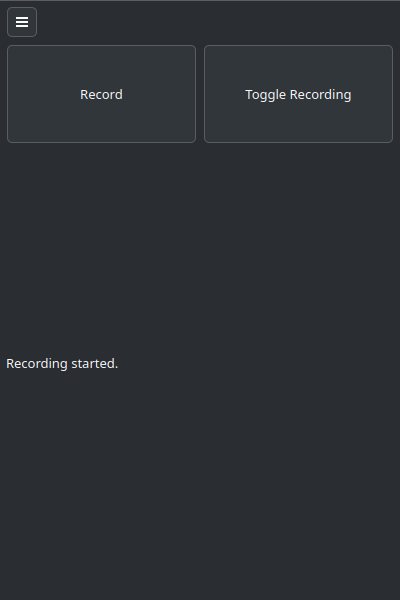
\includegraphics[width=\textwidth]{assets/mainwindow_january.png}
    \caption{Main Window of the Qt application}
    \label{fig:mainwindow_january}
\end{minipage}
\hfill
\begin{minipage}{0.45\textwidth}
    \centering
    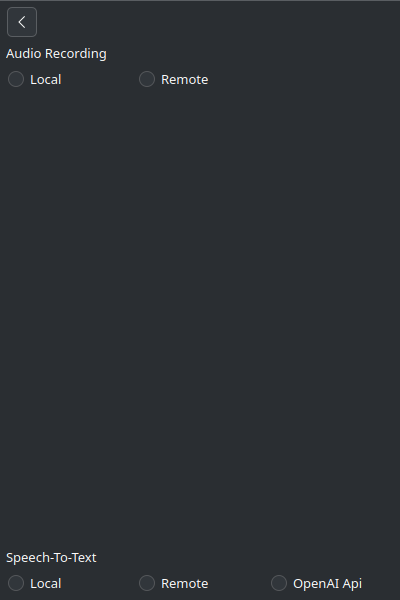
\includegraphics[width=\textwidth]{assets/settings_january.png}
    \caption{Settings Window of the Qt application}
    \label{fig:settings_january}
\end{minipage}
\end{figure}

\section{Raspberry Pi Integration}
\subsection{Operating System Selection}
Alpine Linux proved to be the best choice for running
the system on Raspberry Pi hardware. Its minimal design and
stripped-down core components made it ideal for our embedded
application. By using musl libc and BusyBox instead of traditional
tools, Alpine runs with much lower RAM and storage overhead
than standard Linux distributions. This efficiency was critical since
real-time audio processing and language models already tax the Pi's
resources. The simple apk package manager made installing dependencies straightforward,
while keeping the system lean.
